%%%%%%%%%%%%%%%%%%%%%%%%%%%%%%%%%%%%%%%%%%%%%%%%%%%%%%%%%%%%%%%%%%%%%%%%%%%%%%%%%%%%%%%%%%%%%%%%%%%%
% ==================================================================================================
% --------------------------------------------------------------------------------------------------
\chapter{Implementation}
This appendix contains implementation details.
%%%%%%%%%%%%%%%%%%%%%%%%%%%%%%%%%%%%%%%%%%%%%%%%%%%%%%%%%%%%%%%%%%%%%%%%%%%%%%%%%%%%%%%%%%%%%%%%%%%%
\section{Parallel Fitting}
Speed of model fitting is a significant factor during development, particularly considering optimization of so-called hyperparameters. Faster training yields more model iterations, which inevitably bear improvements. In order to efficiently estimate the logistic regression parameters for all voxels -- which are modelled independently -- it is helpful to compute these in parallel.
\par...\par
The first step in such optimization schemes is to scale the feature data by the classification labels $\C$,
\begin{equation}
  \Y_{\C=1} \leftarrow -\Y_{\C=1}.
\end{equation}
\par...\par
The computations of the update include
\begin{align*}
  \eta = 
\end{align*}
%%%%%%%%%%%%%%%%%%%%%%%%%%%%%%%%%%%%%%%%%%%%%%%%%%%%%%%%%%%%%%%%%%%%%%%%%%%%%%%%%%%%%%%%%%%%%%%%%%%%
\section{Revised Manual Segmentations}
Since the reported performance of an automatic segmentation algorithm depends on the manual segmentations to which it is compared, it is important to obtain good manual segmentations. Unfortunately, the original manuals in the MS 2008 Segmentation Challenge contained obvious artifacts and inconsistencies, as shown at left in Figure \ref{fig:m08-rev}. Therefore, it was deemed necessary to revise these manuals. To do this, the Editor module from the 3D Slicer imaging platform \cite{Fedorov2012} was used\footnote{3D Slicer Editor tool documentation is available here: \hreftt{https://www.slicer.org/wiki/Documentation/4.6/Modules/Editor}.}, including the Wand, Paint, and Erase functions. Figure \ref{fig:m08-rev-slicer} shows the user interface, while the resulting revisions are shown at right in Figure \ref{fig:m08-rev}.
\begin{figure}
  \centering
  \begin{minipage}{6cm}
    \begin{subfigure}{\textwidth}
      \centering\subcaption{Original}\label{fig:m08-rev-o}
      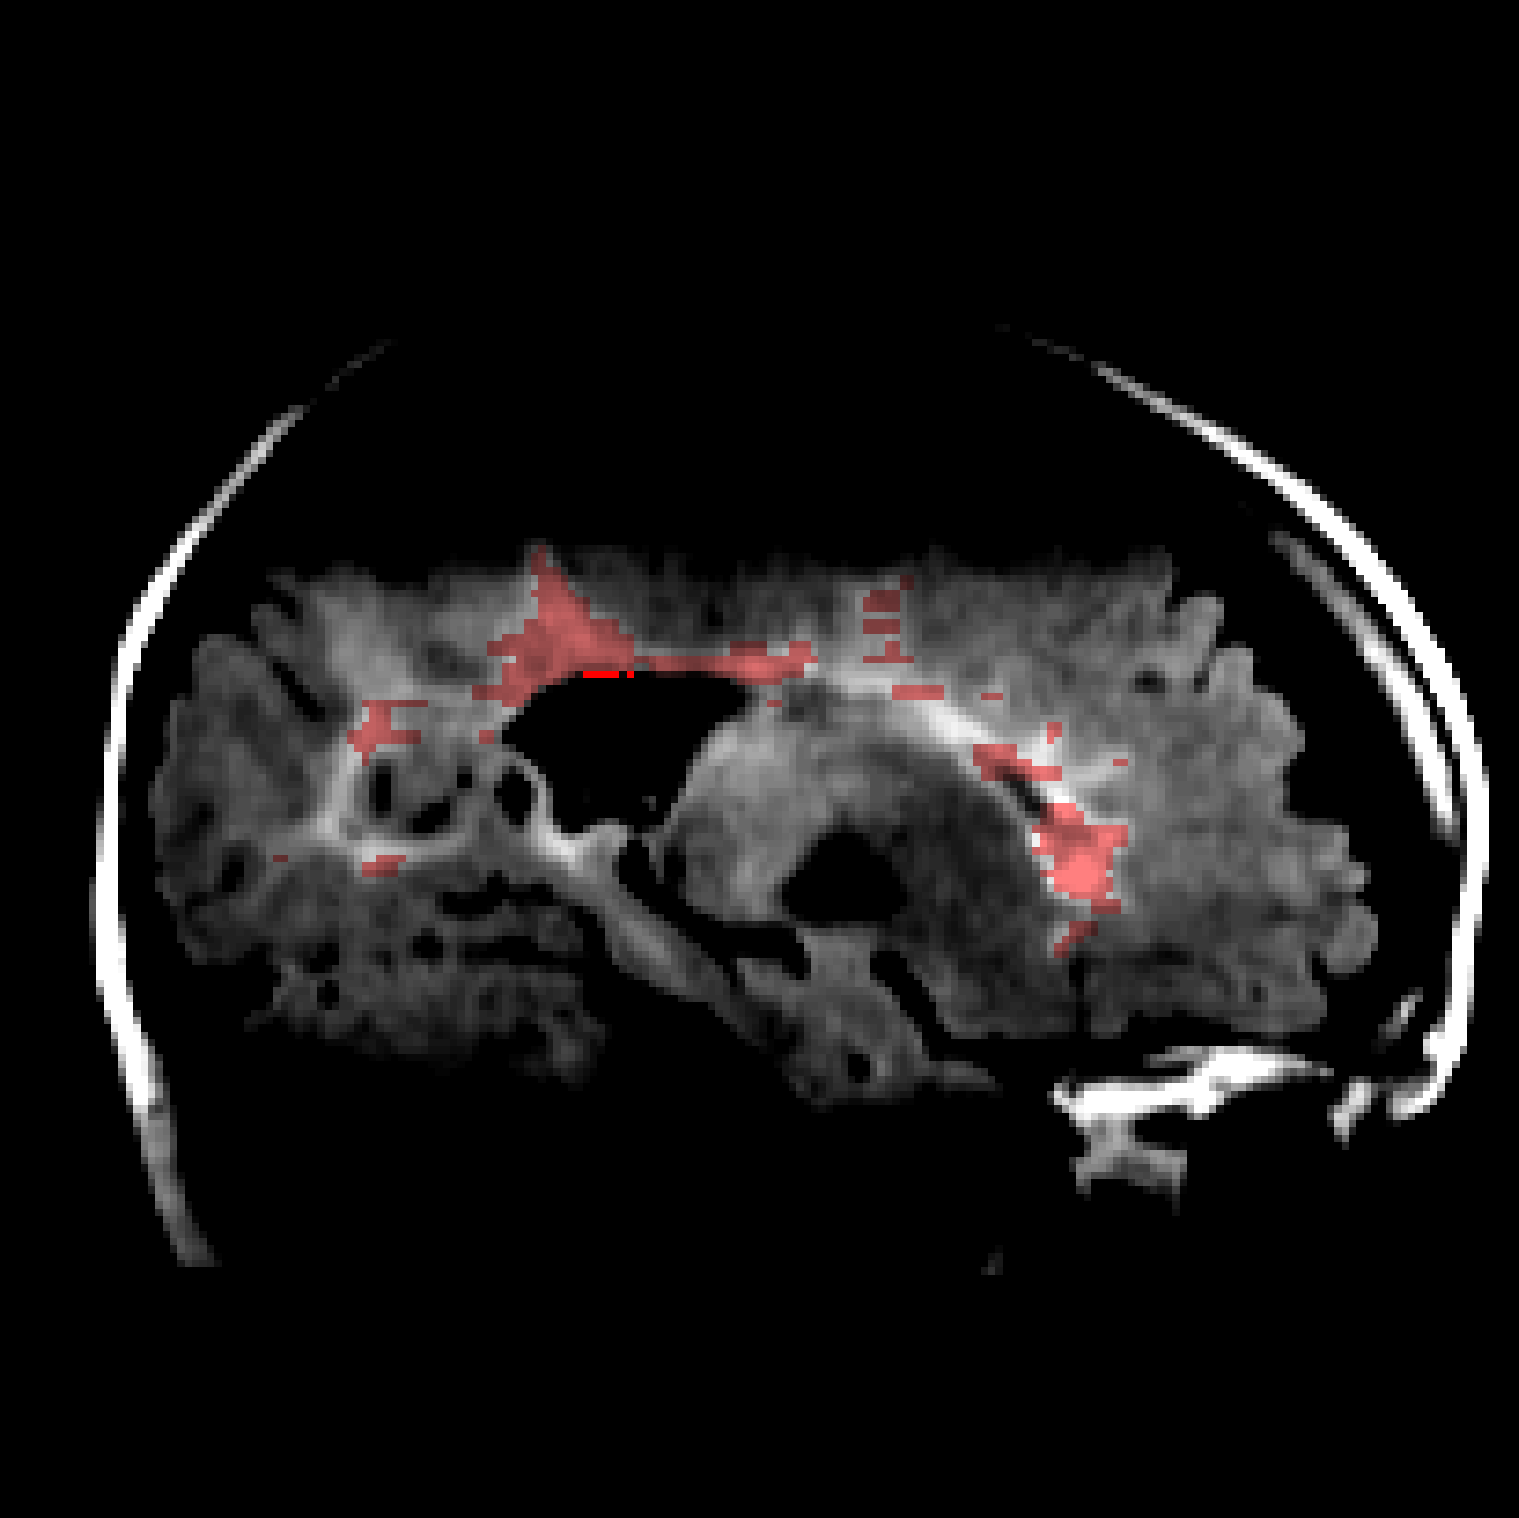
\includegraphics[height=6cm]{m08rev-01-d2-z146-o}\\[0.2em]
      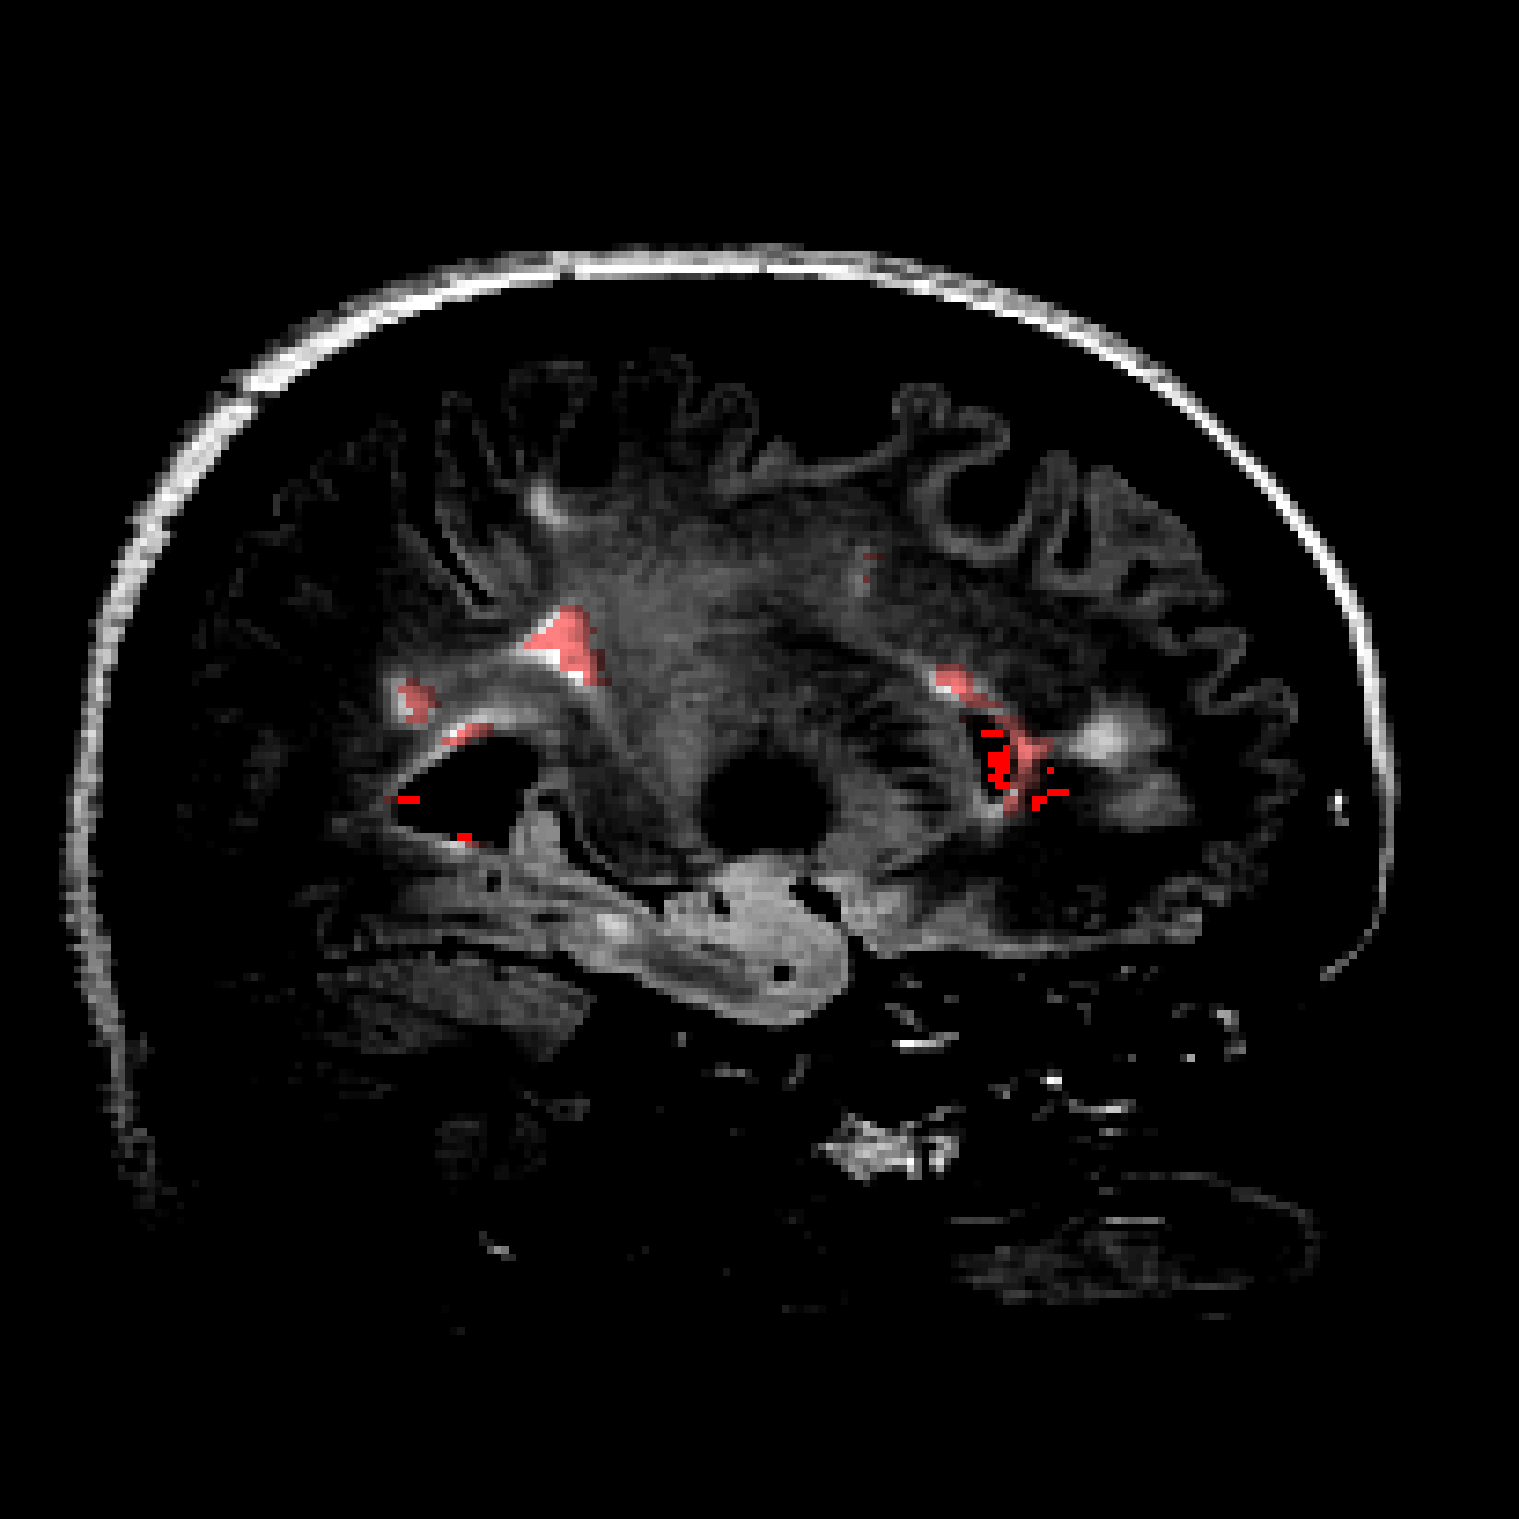
\includegraphics[height=6cm]{m08rev-05-d2-z107-o}\\[0.2em]
      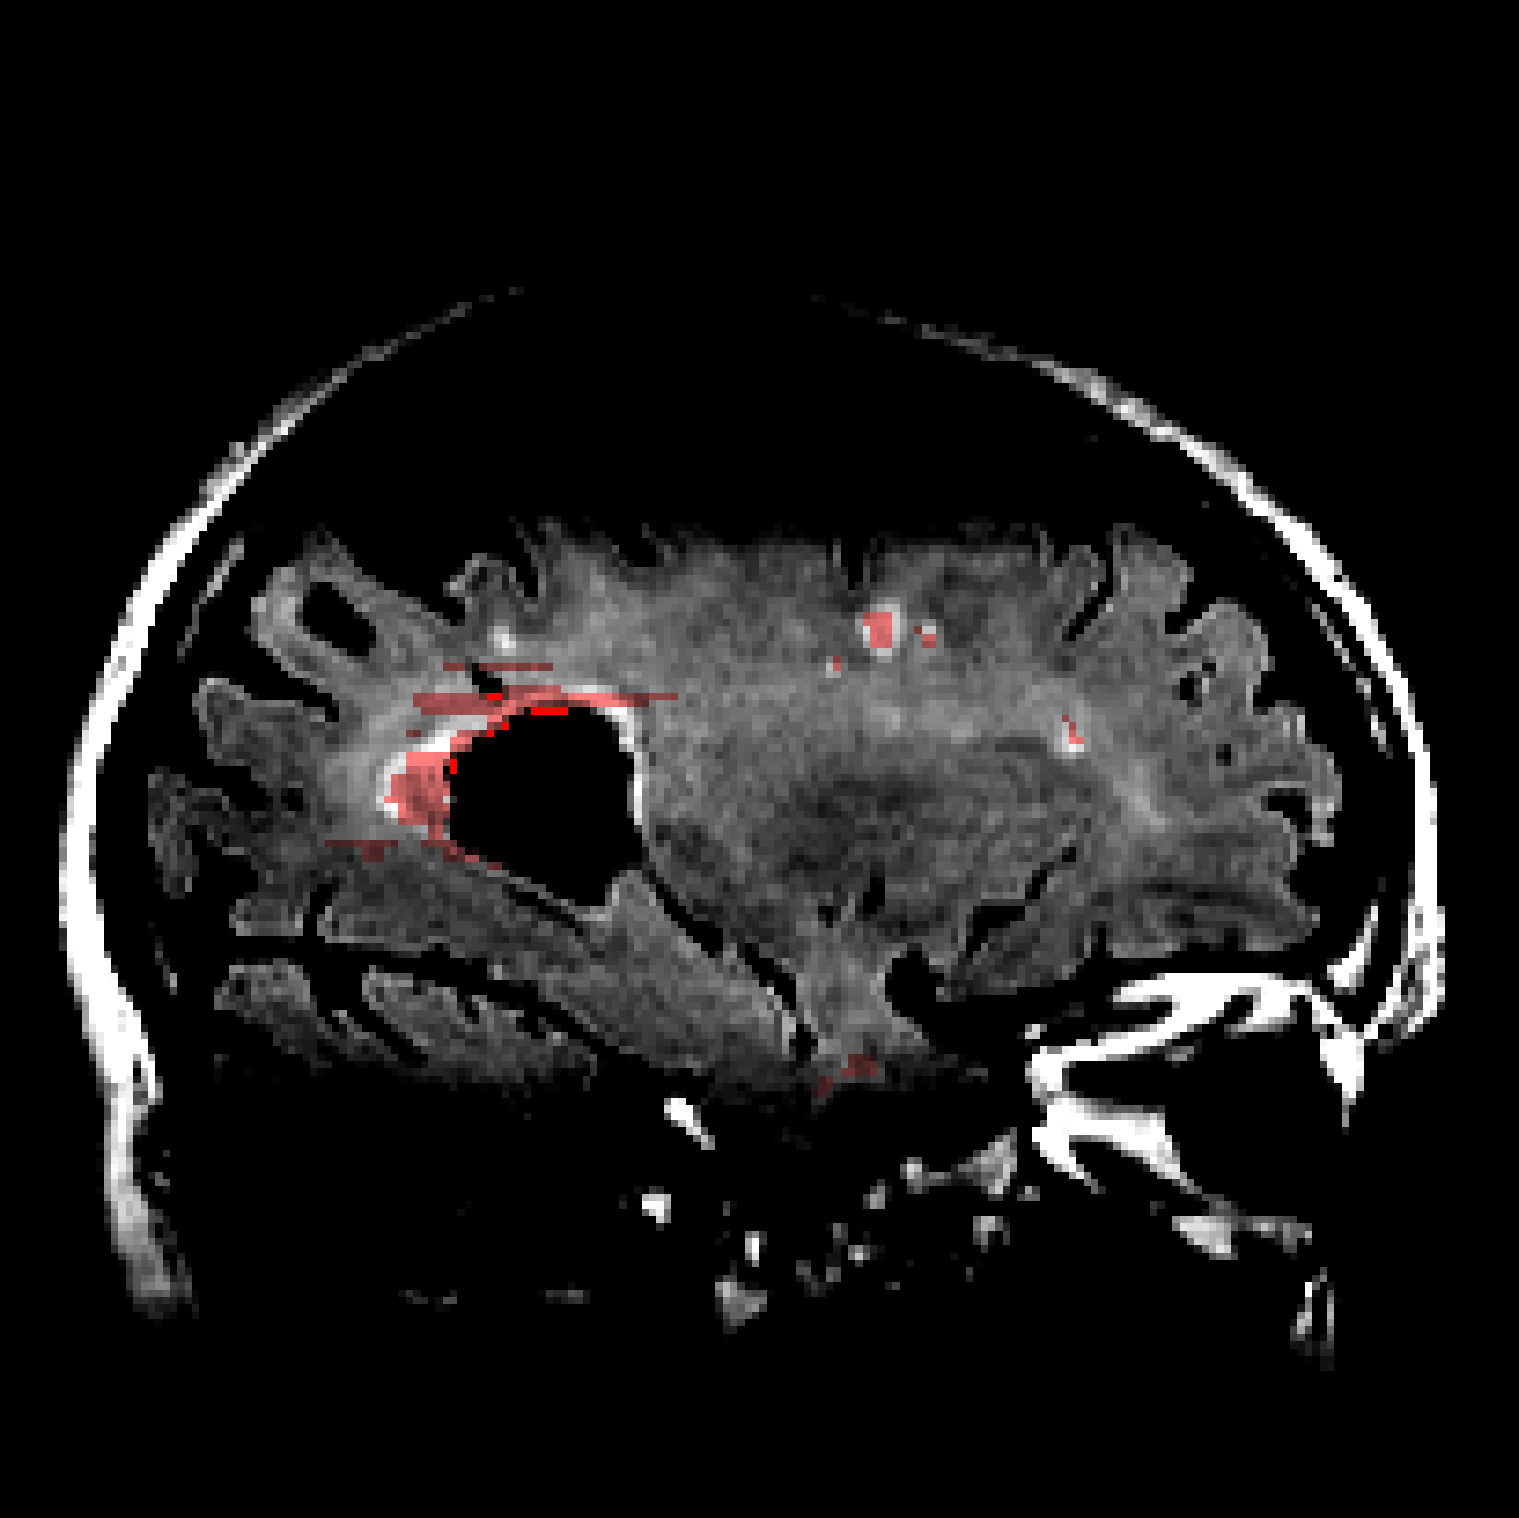
\includegraphics[height=6cm]{m08rev-06-d2-z101-o}
    \end{subfigure}
  \end{minipage}
  \begin{minipage}{6cm}
    \begin{subfigure}{\textwidth}
      \centering\subcaption{Revision}\label{fig:m08-rev-r}
      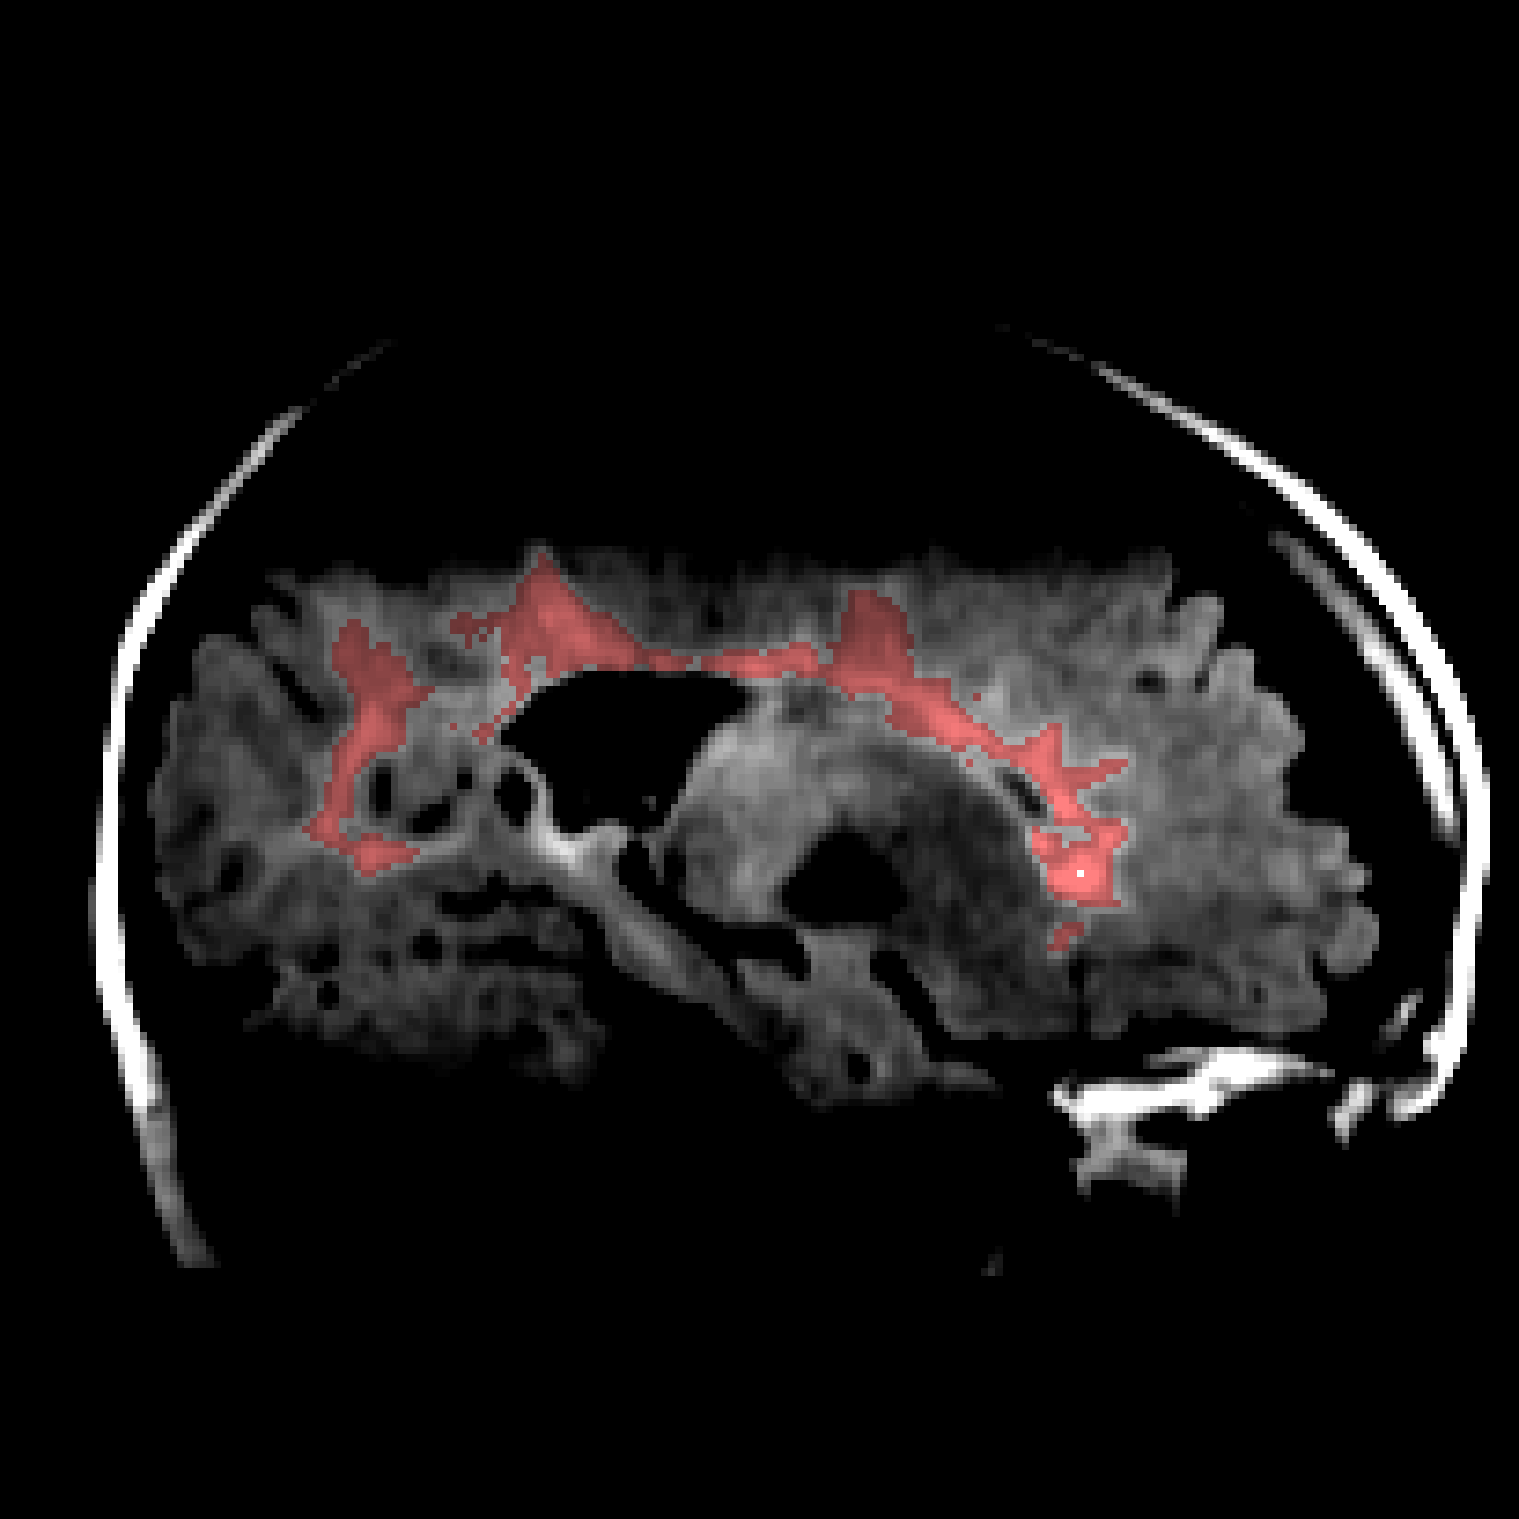
\includegraphics[height=6cm]{m08rev-01-d2-z146-r}\makebox[0pt][r]{\textcolor{white}{ CHB 01 }}\\[0.2em]
      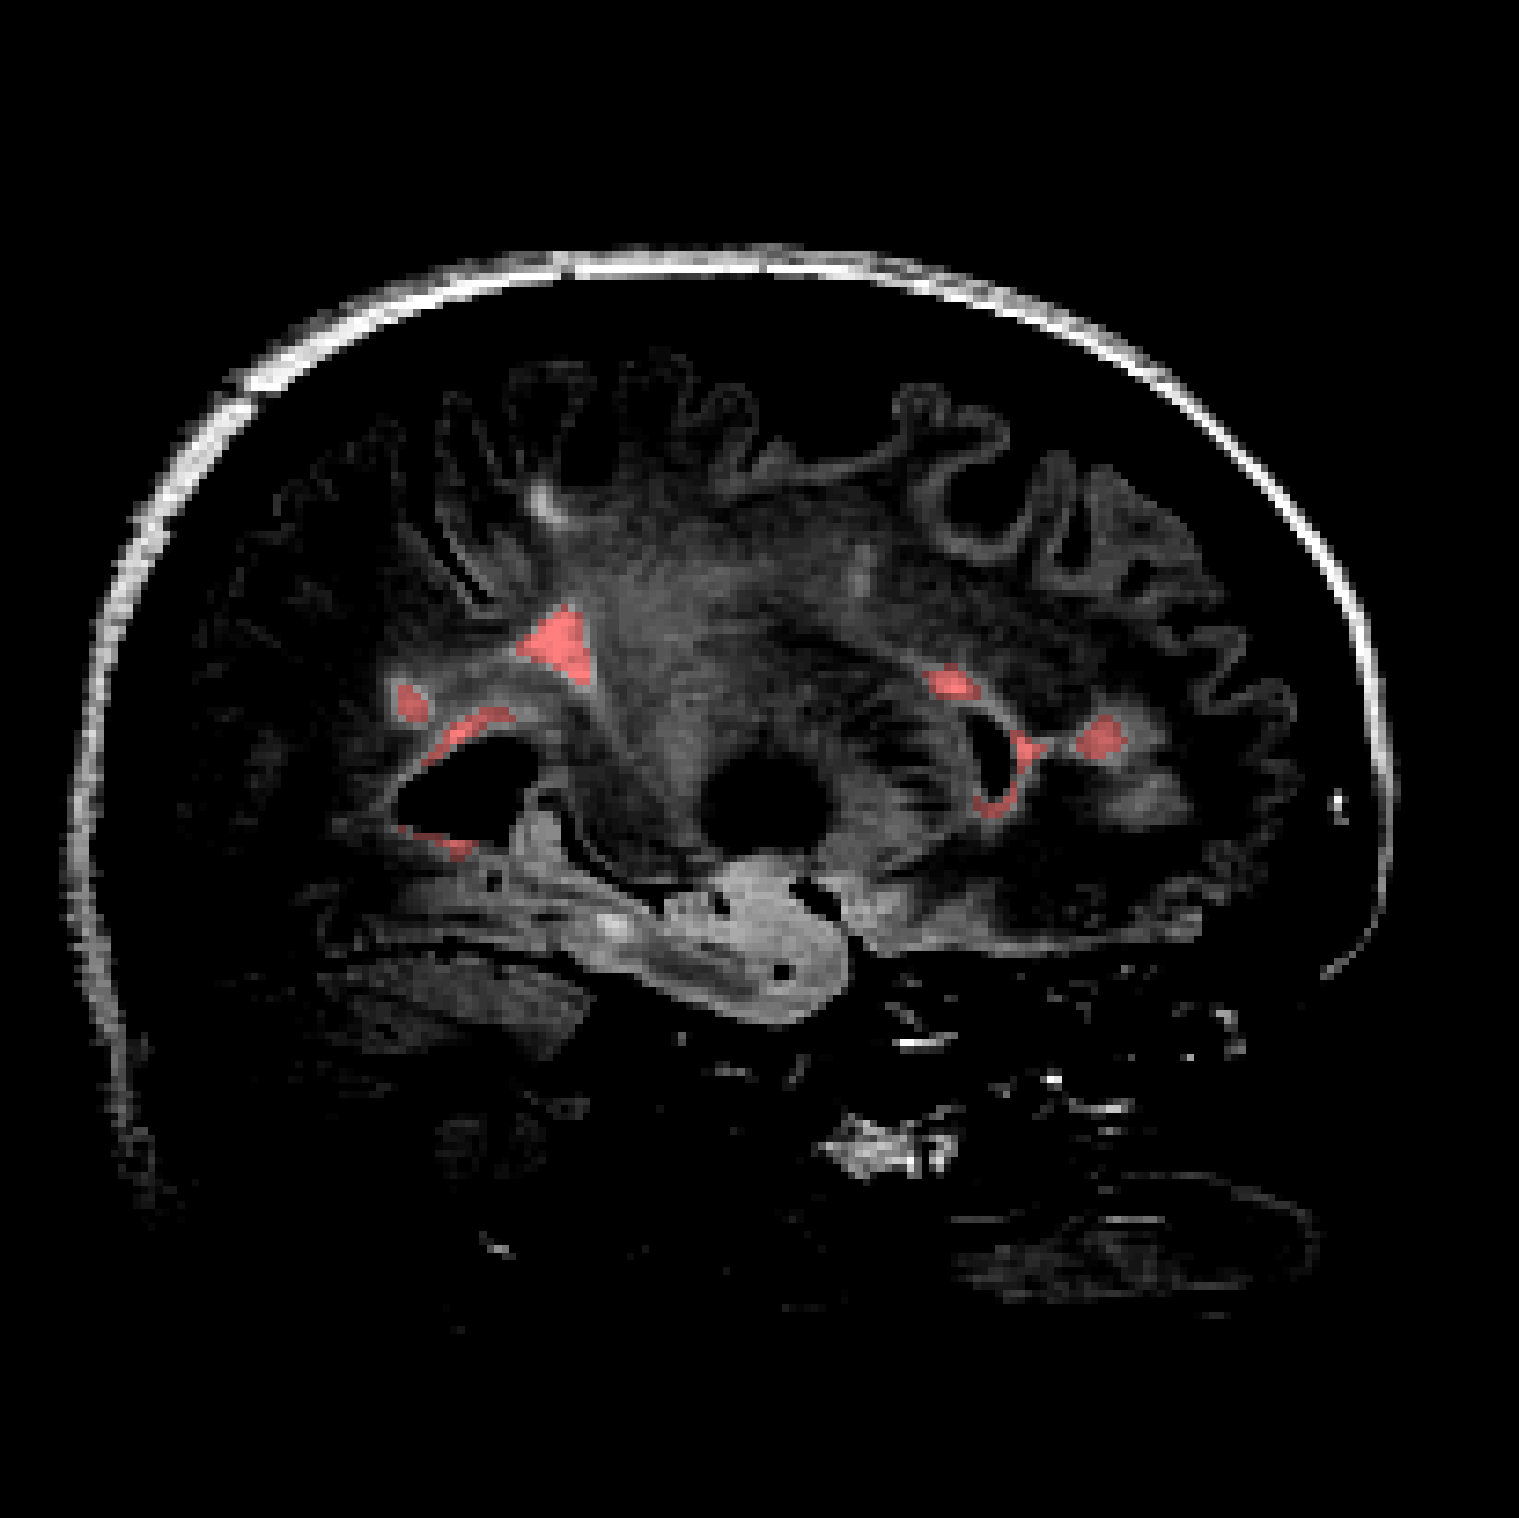
\includegraphics[height=6cm]{m08rev-05-d2-z107-r}\makebox[0pt][r]{\textcolor{white}{ CHB 05 }}\\[0.2em]
      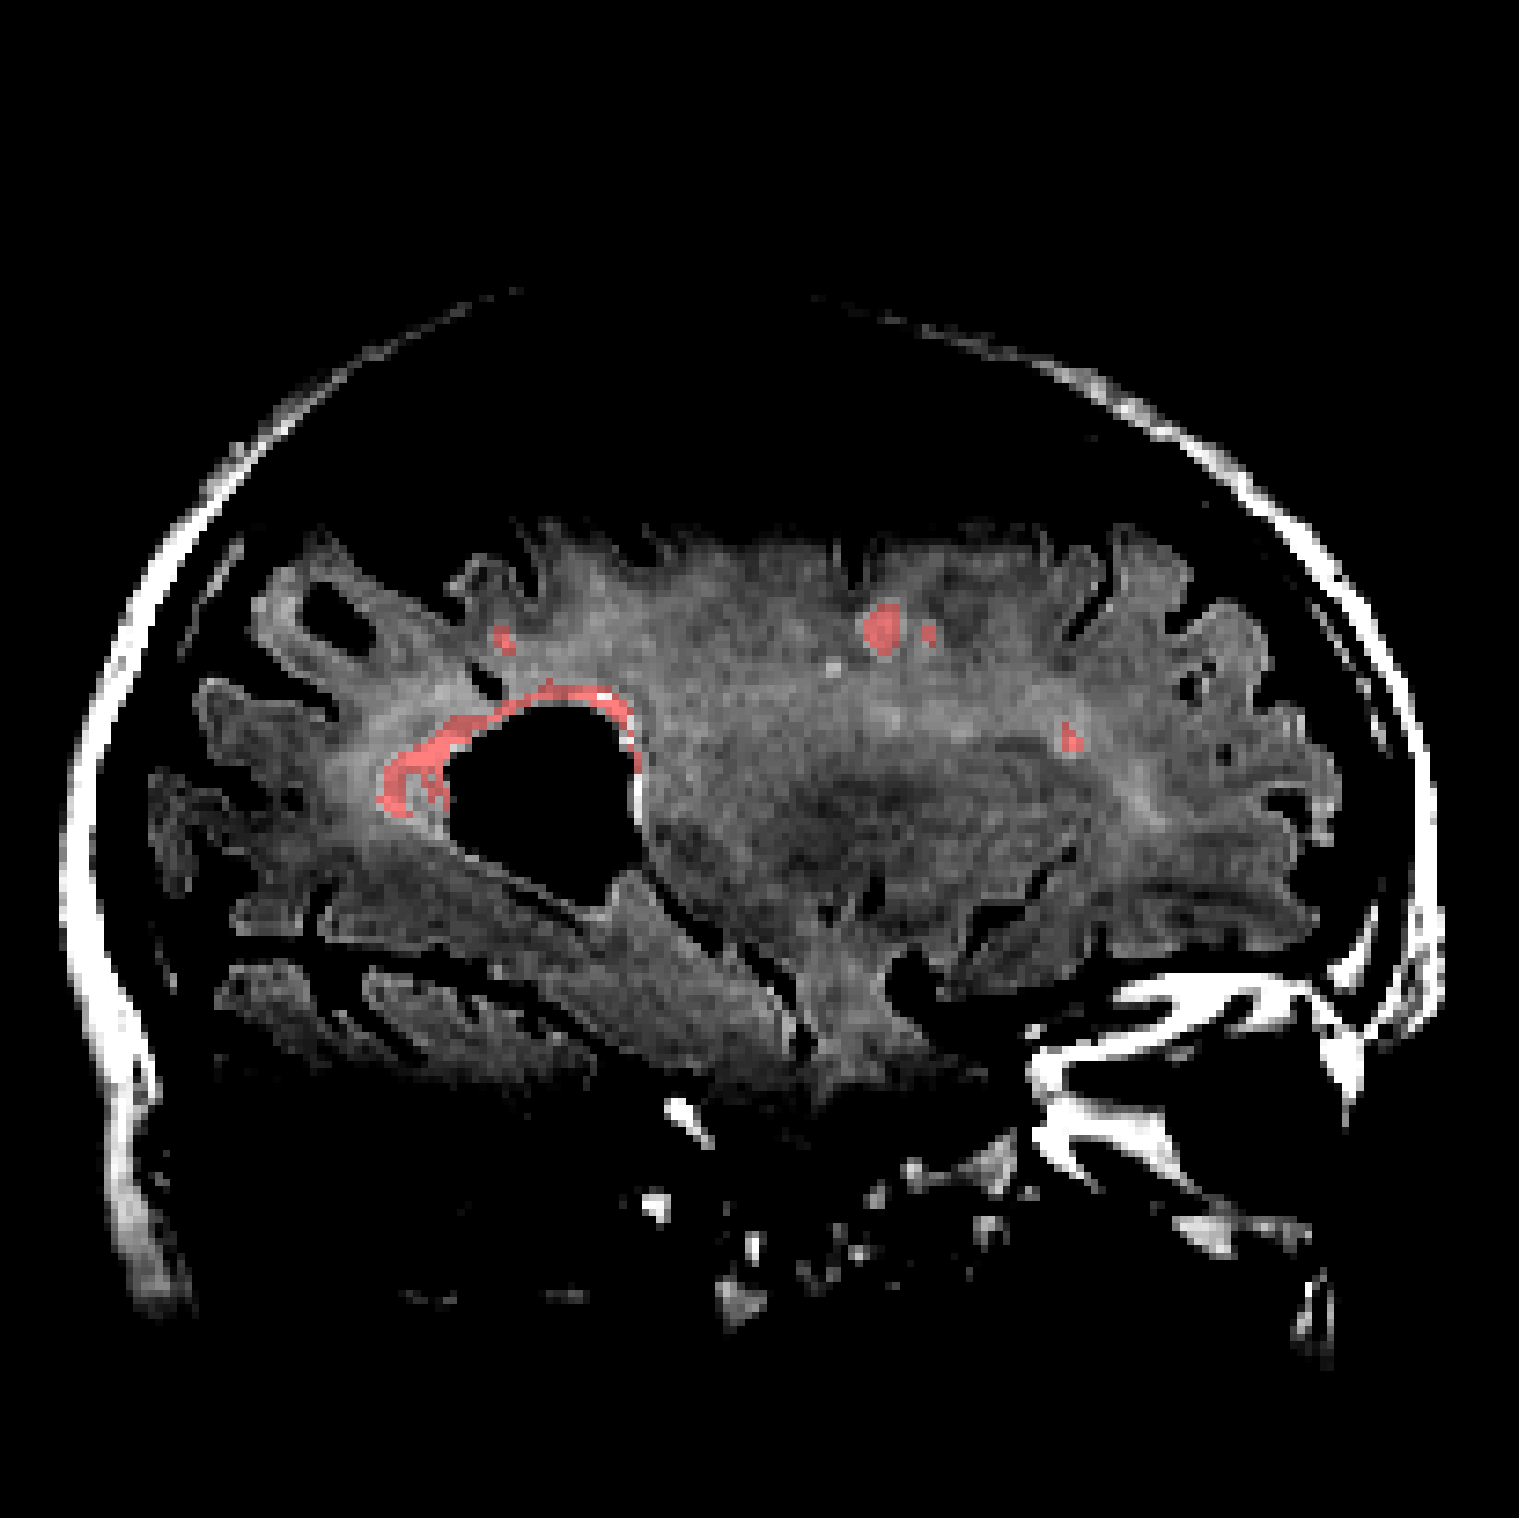
\includegraphics[height=6cm]{m08rev-06-d2-z101-r}\makebox[0pt][r]{\textcolor{white}{ CHB 06 }}
    \end{subfigure}
  \end{minipage}
  \caption{Example revisions to the manual segmentations for the MS 2008 challenge dataset.}
  \label{fig:m08-rev}
\end{figure}
\begin{figure}
  \centering
  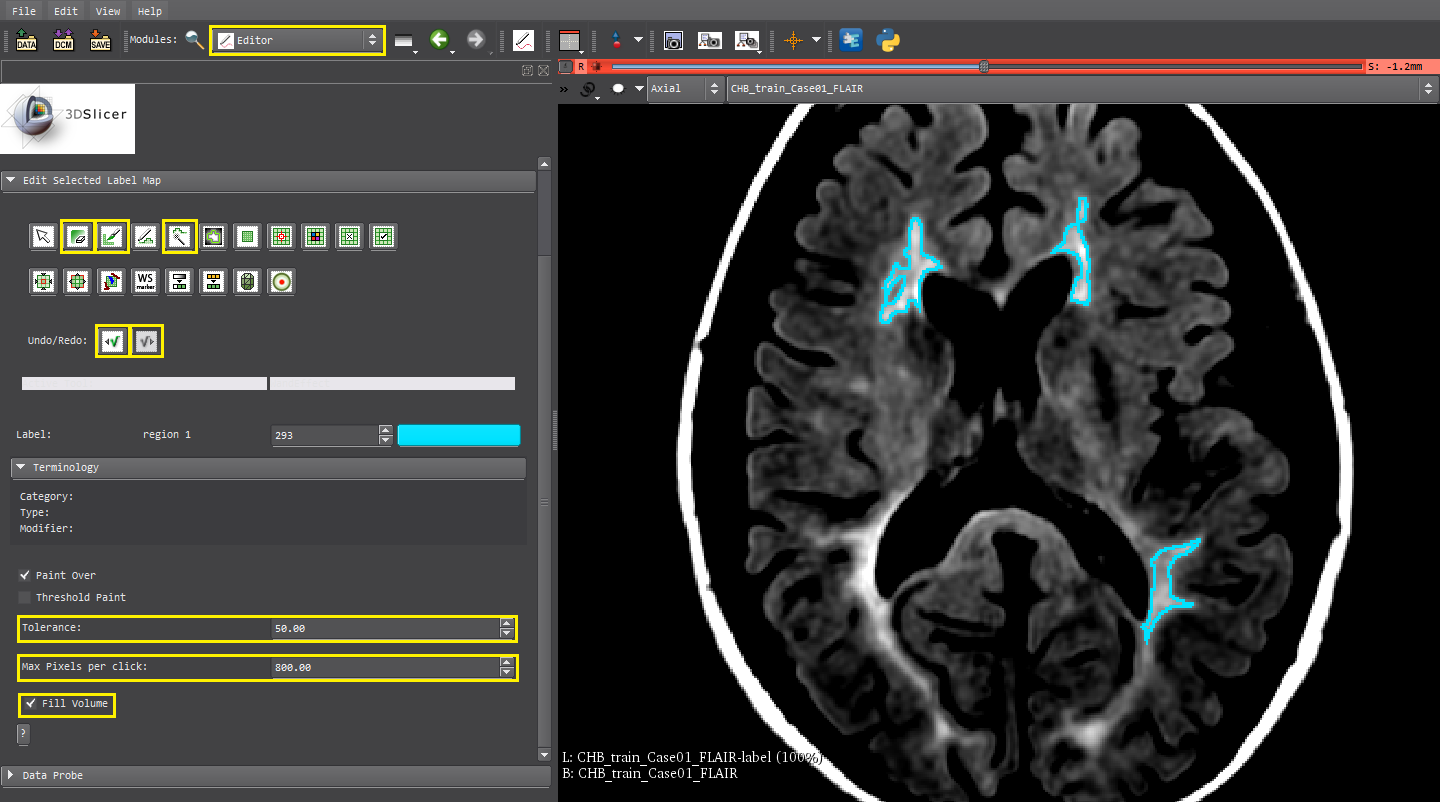
\includegraphics[width=\textwidth]{m08rev-slicer.png}
  \caption{3D Slicer user interface for performing in-house manual segmentations revisions. The tools and parameters used are highlighted in yellow, while the segmentation (in-progress) is shown in blue.}
  \label{fig:m08-rev-slicer}
\end{figure}

%%%%%%%%%%%%%%%%%%%%%%%%%%%%%%%%%%%%%%%%%%%%%%%%%%%%%%%%%%%%%%%%%%%%%%%%%%%%%%%%%%%%%%%%%%%%%%%%%%%%

% --------------------------------------------------------------------------------------------------
% ==================================================================================================
%%%%%%%%%%%%%%%%%%%%%%%%%%%%%%%%%%%%%%%%%%%%%%%%%%%%%%%%%%%%%%%%%%%%%%%%%%%%%%%%%%%%%%%%%%%%%%%%%%%%
